%! Author = Adrian Helberg
%! Date = 21.09.2020

% Preamble
\documentclass[11pt]{article}
% Packages
\usepackage{ngerman}
\usepackage{amsmath}
\usepackage{url}
\usepackage{graphicx}
\usepackage{float}
\usepackage{enumitem,amssymb}
\newlist{todolist}{itemize}{2}
\setlist[todolist]{label=$\square$}
\usepackage{pifont}
\newcommand{\cmark}{\ding{51}}%
\newcommand{\xmark}{\ding{55}}%
\newcommand{\done}{\rlap{$\square$}{\raisebox{2pt}{\large\hspace{1pt}\cmark}}%
\hspace{-2.5pt}}
\newcommand{\wontfix}{\rlap{$\square$}{\large\hspace{1pt}\xmark}}

\title{\textbf{Exposé} zur Bachelorarbeit von Adrian Helberg bei Prof. Dr. Jenke}

% Document
\begin{document}
    \maketitle

    \section{Problemstellung}

    Effizientes Objektdesign und -modellierung sind entscheidende Kernkompetenzen in verschiedenen Bereichen der
    digitalen Welt.
    Da die Erstellung geometrischer Objekte unintuitiv ist und ein großes Maß an Erfahrung und Expertise
    erfordert, ist dieses stetig wachsende Feld für Neueinsteiger nur sehr schwer zu erschließen.
    Die Forschung liefert hierzu einige Arbeiten zur \textbf{prozeduralen Modellierung}, um digitale Inhalte schneller
    und automatisiert zu erstellen.
    Gerade wenn es um die Darstellung natürlicher Umgebung geht, ist die Erstellung von ähnlichen Objekten, wie
    zum Beispiel verschiedene Bäume derselben Gattung eines Waldes, ein schwieriges Problem.
    Kleine Änderungen in prozeduralen Systemen können zu großen Veränderungen der Ergebnisse führen.
    Darum beschäftigt sich die \textbf{inverse prozedurale Modellierung} unter Anderem mit dem Inferieren von Regeln
    und Mustern aus gegeben Objekten, um diese nach bestimmten Regeln zu modellieren.
    Ein wichtiges Werkzeug hierbei ist die Verwendung einer \textbf{formalen Grammatik}, eine fundamentale Datenstruktur
    der Informatik, um Strukturen zu beschreiben.
    Eine spezielle Untergruppe sind die \textbf{L-Systeme}, die häufig bei der Beschreibung
    von Verzweigungsstrukturen und Selbstähnlichkeit zum Einsatz kommen.\\~\\
    Die Bachelorarbeit soll sich mit der Erstellung eines prozeduralen Systems zur Synthese von Ähnlichkeitsabbildern
    beschäftigen.
    Hierzu soll über eine Benutzerschnittstelle eine Struktur erzeugt werden, aus der ein parametrisiertes L-Systems
    inferiert werden kann, das dann zur Generierung von ähnlichen Strukturen genutzt werden kann.

    \subsection{Konzepte und Ideen}
    Im Folgenden wird auf die Methodik zum Ableiten eines L-Systems eingegangen und Konzepte und eigene Lösungsansätze
    präsentiert.

    \begin{figure}[H]
        \centering
        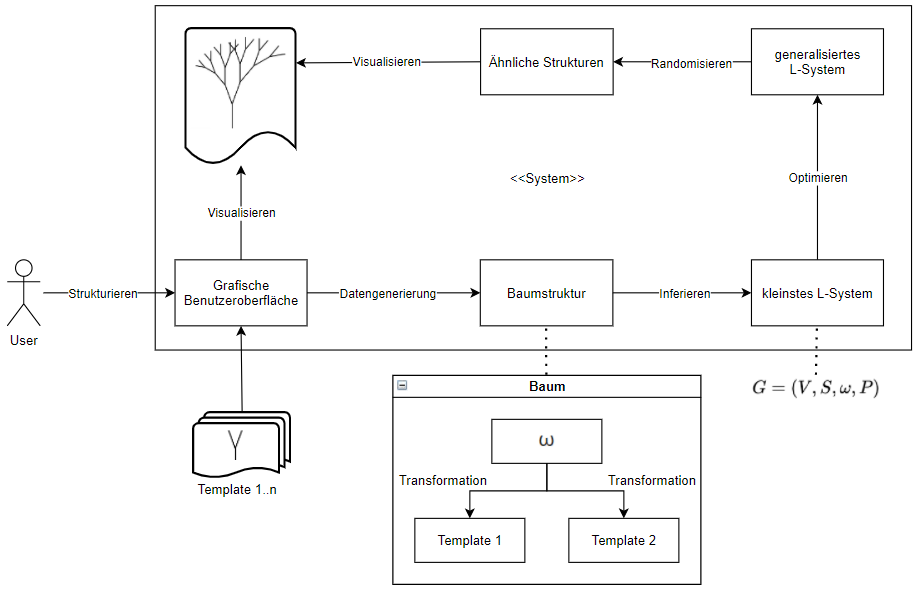
\includegraphics[width=14cm]{../images/System.PNG}
        \caption[Systemarchitektur]{Architektur des Systems mit einigen Datenstrukturen}
    \end{figure}

    \subsubsection{System}
    Ziel des Systems ist die Erstellung von Ähnlichkeitsabbildern einer Struktur, die über eine grafische
    Benutzeroberfläche erstellt wird.

    \newpage

    \subsubsection{Überblick}
    \textit{Abbildung 1 zeigt, wie das o.g. System aufgebaut ist}:
    \begin{itemize}
        \item[I.] \underline{Strukturieren}: Der Benutzer nutzt die grafische Benutzerschnittstelle, um aus
        einzelnen, atomaren Strukturen (\textbf{Templates}) eine zusammenhängende Struktur zu erstellen.
        Neben der Position der Templates können auch Parameter wie Rotation angepasst
        werden.
        \item[II.] \underline{Visualisieren}: Das Ergebnis der Strukturierung ist jederzeit sichtbar.
        Einfache Liniensegmente können mit einem \textbf{Turtle-Algorithmus} gezeichnet werden.
        \item[III.] \underline{Datengenerierung}: Das Ergebnis der Strukturierung wird in einer Baumstruktur
        organisiert, in der jeder Knoten einem bestimmten Template entspricht und die zugehörigen Kanten die
        geometrischen Transformationen relativ zum Elternknoten beschreibt.
        \item[IV.] \underline{Inferieren}: Aus der Baumstruktur kann eine formale Grammatik in Form eines kleinen
        L-Systems abgeleitet werden, indem identische topologische Strukturen (Unterbäume) gefunden werden können.
        \item[V.] \underline{Optimieren}: Hier werden ähnliche Produktionsregeln des L-Systems mithilfe einer
        \textbf{Kostenfunktion}\footnote[1]{Die Kostenfunktion setzt sich sowohl aus der Länge der Grammatik, als
        auch der Distanz von der alten zur neuen, generalisierten Grammatik nach dem Merge zusammen} zusammengefasst
        (\textit{engl. Merge}), um diese mit nicht-deterministischen Regeln und Rekursion zu generalisieren.
        \item[VI.] \underline{Randomisieren}: Jedes Symbol der Grammatik nimmt eine Liste an Parametern entgegen, die
        in diesem Schritt nach bestimmten Kriterien pseudo-randomisiert werden, um Variationen zu erstellen und
        anschließend zu visualisieren.
    \end{itemize}

    \newpage

    \subsection{Einführung}
    \textit{Die Einführung in das Themas könnte wie folgt aussehen}:\\~\\
    Mit der Digitalisierung der Welt erlangt die Erstellung von digitalen Inhalten, wie 3D Modelle für Computerspiele,
    Webdesigns oder Visualisierung von Architektur, zunehmend an Bedeutung.
    Darum werden Verfahren gesucht, um Objekte dieser Felder formal zu beschreiben und somit kodifizierbar
    (\textit{engl. codify}) zu machen.
    Hierbei bilden sich folgende Klassen heraus:

    \begin{itemize}
        \item \textbf{Modellierung}: Um einen physikalischen Körper in ein digitales Objekt zu überführen, wird mithilfe
        von Abstraktion (oder Modellierung) ein mathematisches Modell erstellt, das diesen Körper formal beschreibt.
        3D Grafiksoftware, wie Blender~\cite{blender}, wird genutzt um geometrische Körper zu modellieren, texturieren
        und zu animieren.
        \item \textbf{Prozedurale Modellierung}: \textit{"`It encompasses a wide variety of generative techniques that
        can (semi-−)automatically produce a specific type of content based on a set of input
        parameters."'}~\cite{1} \\
        "`Prozedurale Modellierung beschreibt generative Techniken, die \\(semi-)automatisch spezifische, digitale
        Inhalte anhand von deskriptiven Parametern erzeugen"' (\textit{Übersetzt durch den Autor})
        \item \textbf{Inverse prozedurale Modellierung (IPM)}:\textit{Aliaga et al.}~\cite{2}
        spricht bei der inversen prozeduralen Modellierung von dem Finden einer prozeduralen Repräsentation von
        Strukturen bestehender Modelle.
    \end{itemize}
    Die Modellierung mithilfe von Grafiksoftware ist eine vergleichbar händische, langwierige Erstellung von
    Objekten.
    Hierbei hat der Designer (= Modellierer) die volle Kontrolle über die Strukturen des Objektes.\\
    Bei der prozeduralen Modellierung werden spezifische Strukturen eines zu erstellenden physikalischen Objektes
    generalisiert und meist über eine Grammatik und globale Parameter abgebildet.
    Während bei der klassischen Modellierung die menschliche Intuition und bei der prozeduralen Modellierung eine
    parametrisierte Grammatik vorausgesetzt wird, arbeitet IPM mit bestehenden Modellen und extrahiert ("`lernt"')
    die Strukturen des Objektes, die automatisch in eine formale Grammatik überführt werden können.
    Die Generierung von prozeduralen Modellen ist ein wichtiges, offenes Problem~\cite{2}.

    \newpage

    Aktuelle Ansätze sind:
    \begin{itemize}
        \item Segmentierung von geometrischen Objekten in Ähnlichkeitsgruppen, um Muster (\textit{engl. Patterns}) zu
        erkennen
        \item Kontrollierte Generierung durch Finden optimaler Prameter und Regeln
    \end{itemize}

    \subsection{Vorangehende Arbeiten}
    \textit{Dieses Kapitel beschreibt die relevanten Themen der Bachelorarbeit und stellt einige wissenenschaftliche
    Quellen vor:}
    \begin{itemize}
        \item (Inverse) Prozedurale Modellierung~\cite{2} und~\cite{1}:\\Siehe Kapitel 1.2 Einführung
        \item Logo-Turtle-Algorithmus~\cite{3}:\\ Der Logo-Turtle-Algorithmus bezeichnet eine Methode zur Generierung
        von Bildern mithilfe einer Zeichenkette, deren Symbole jeweils für einen bestimmten Befehl zur Steuerung einer
        "`Schildkröte"' (\textit{engl. turtle}) stehen.
        Die Visualisierung von Fraktalen und natürlicher Vegetation stellen zwei Beispiele für die Anwendung dar.
        \item L-System~\cite{5}:\\ L-Systeme sind spezielle, formale Grammatiken zur Beschreibung von
        natürlicher Vegetation.
        Lindenmayer führte dieses Stringersetzungssystem ein, um Zellteilung formal zu beschreiben.
    \end{itemize}

    \newpage

    \begin{itemize}

    \end{itemize}

    \section{Ablauf}
    \begin{itemize}
        \item Erarbeitung eines Software-/Harwarestacks
        \item Erstellung eines Projektplans mit Arbeitspaketen
        \item Herausarbeiten einer Softwarearchitektur
        \item Prototypische Entwicklung eines Systems zur Erstellung "`ähnlicher"' 2D-Strukturen anhand eines
        Input-Bildes, das mit einer grafischer Oberfläche erstellt wird
        \item Schriftliche Ausarbeitung der Ergebnisse
        \item Zweiwöchige Meilensteine mit Besprechungen (Videokonferenz)
        \item Phasen:
        \begin{itemize}
            \item Vorbereitung
            \item Literaturstudium
            \item Problemstudium
            \item Praktische Arbeit
            \item Schriftliche Arbeit
        \end{itemize}
    \end{itemize}

    \section{Zeitplan}
    \begin{todolist}
        \item[\done] bis 29.08.2020: Erarbeitung Basisquelle
        \item[\done] 14.09.2020: Kennenlerngespräch, erstes Themengespräch
        \item[\done] bis 28.09.2020: Version 1.0 des Exposés
        \item[\done] bis 13.10.2020: Einigung auf eine neue Fragestellung
        \item[\done] bis 18.10.2020: Version 2.0 des Exposés, Zweitgutachter auswählen
        \item bis 23.10.2020: Problemstudium, Anmeldung der Bachelorarbeit, Ausarbeitung des Software-/Hardwarestacks
        \item bis 26.10.2020: Erstellung des Projektplans mit Arbeitspaketen
        \item ab 26.10.2020: Bearbeitung des praktischen Teils der Bachelorarbeit, paralleler Beginn des schriftlichen Teils
    \end{todolist}

    \listoffigures

    ~\nocite{*}
    \bibliography{literature_2}
    \bibliographystyle{plain}

\end{document}